\documentclass{article}
% The preceding line is only needed to identify funding in the first footnote. If that is unneeded, please comment it out.
\usepackage{amsmath,amssymb,amsfonts}
\usepackage{graphicx}

%%% MOJE
%\DeclareGraphicsExtensions{.ps, .eps}
%\usepackage[slovak]{babel}
\usepackage[utf8]{inputenc} 

\newcommand{\dif}{\, \mathrm{d}}	% diferencia (na derivacie)
\newcommand{\difp}{\partial}		% parc. diferencia 
\newcommand{\dxdt}[2]{\frac{\mathrm{d} #1}{\mathrm{d} #2}}
\newcommand{\dxdtp}[2]{\frac{\partial #1}{\partial #2}}
\newcommand{\un}[1]{\, \mathrm{#1}}	% jednotky velicin, v math mode
\newcommand{\E}[1]{\cdot 10^{#1}}
\newcommand{\degree}{^\circ}
\newcommand{\diameter}{\emptyset}
\newcommand{\cpx}{\widehat}		% komplexne fazory
\newcommand{\Ohm}{\Omega}

\newcommand{\myfigtex}[3]
{
    \begin{figure}[!ht]
        \centering
        \input{#1}
        \caption{#2}
        %\label{fig:#3}
        #3
    \end{figure}
}

\pagestyle{empty}
\begin{document}

%% XCircuit output "obr/Tzap.tex" for LaTeX input from obr/Tzap.ps
\def\putbox#1#2#3#4{\makebox[0in][l]{\makebox[#1][l]{}\raisebox{\baselineskip}[0in][0in]{\raisebox{#2}[0in][0in]{\scalebox{#3}{#4}}}}}
\def\rightbox#1{\makebox[0in][r]{#1}}
\def\centbox#1{\makebox[0in]{#1}}
\def\topbox#1{\raisebox{-0.60\baselineskip}[0in][0in]{#1}}
\def\midbox#1{\raisebox{-0.20\baselineskip}[0in][0in]{#1}}
   \scalebox{0.8}{
   \normalsize
   \parbox{3.33333in}{
   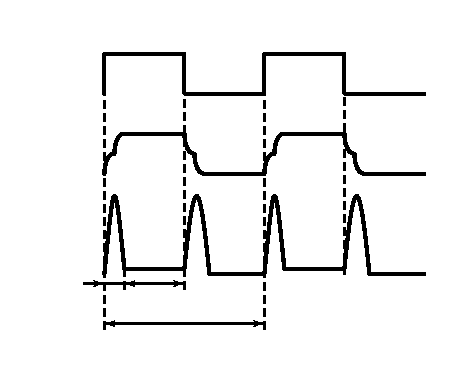
\includegraphics[scale=1.25]{obr}\\
   % translate x=367 y=487 scale 0.30
   \putbox{0.77in}{0.44in}{1.20}{$t_{on}$}%
   \putbox{1.11in}{0.44in}{1.20}{$T_{on,\,act}$}%
   \putbox{1.31in}{0.11in}{1.20}{$T_{per}$}%
   \putbox{0.90in}{2.61in}{1.20}{ON}%
   \putbox{1.56in}{2.61in}{1.20}{OFF}%
   \putbox{0.23in}{1.61in}{1.20}{$v_{GS}$}%
   \putbox{0.23in}{0.77in}{1.20}{$p$}%
   \putbox{0.06in}{2.27in}{1.20}{control}%
   } % close 'parbox'
   } % close 'scalebox'
   \vspace{-\baselineskip} % this is not necessary, but looks better

\myfigtex{obr}{}{}


\end{document}
